
\documentclass[handout,t]{beamer}
\usepackage[utf8]{inputenc}

\usepackage[alf]{abntex2cite}
\usefonttheme[onlymath]{serif}

\usepackage{graphicx}
\usepackage{caption}
\usepackage{float}
\usepackage{geometry}
\usepackage{amsmath,amssymb,lmodern, lipsum}
\usepackage{url}
\usepackage{pgfpages}
\usepackage{enumerate}
\usepackage{color}
\usepackage{ifthen}
\usepackage{capt-of}
\usepackage{listings}
\usetheme{Berlin}
\usecolortheme{ufrn}
\usepackage{soul}
\usepackage{algorithm,algorithmic}
\usepackage{romannum}
%\usepackage{enumitem}
%\usepackage[table]{xcolor}
\usepackage[export]{adjustbox}



%\usepackage[backend=bibtex]{biblatex}
%\addbibresource{bib/references.bib}

\newcommand{\comment}[1]{}

\setbeamertemplate{caption}[numbered]

\title[Introduction to Artificial Intelligence]{
	(An Almost) No Math Introduction to Deep Learning}
\date{
	\today}
\author[Abhijat Vatsyayan]{
	Abhijat Vatsyayan \inst{1}\\
	%Abhijat Vatsyayan
}

\comment{
	\institute[ Enterprise Information Strategy and Risk Management,]{
		\inst{1}%
		Enterprise Information Stragtegy and Risk Management\\	
		%\href{http://iamap.bms.com}{http://iamap.bms.com}
	}
}
\definecolor{mygreen}{rgb}{0,.5,.1}
\lstset{
	basicstyle=\tiny, 
	%size=10,
	language=Java, 
	commentstyle=\color{mygreen},    % comment style
	escapeinside={\%*}{*)},          % if you want to add LaTeX within your code
	extendedchars=true,              % lets you use non-ASCII characters; for 8-bits encodings only, does not work with UTF-8
	frame=single,	                   % adds a frame around the code
	keepspaces=true,                 % keeps spaces in text, useful for keeping indentation of code (possibly needs columns=flexible)
	keywordstyle=\color{blue},       % keyword style
	morekeywords={*,...},            % if you want to add more keywords to the set
	numbers=left,                    % where to put the line-numbers; possible values are (none, left, right)
	numbersep=5pt,                   % how far the line-numbers are from the code
	numberstyle=\tiny\color{gray}, % the style that is used for the line-numbers
	rulecolor=\color{black},         % if not set, the frame-color may be changed on line-breaks within not-black text (e.g. comments (green here))
	showspaces=false,                % show spaces everywhere adding particular underscores; it overrides 'showstringspaces'
	showstringspaces=false,          % underline spaces within strings only
	showtabs=false,                  % show tabs within strings adding particular underscores
	stepnumber=2,                    % the step between two line-numbers. If it's 1, each line will be numbered
	stringstyle=\color{red}
	}
\begin{document}
	
\setlength{\abovedisplayskip}{0pt}
\setlength{\belowdisplayskip}{0pt}
\setlength{\abovedisplayshortskip}{0pt}
\setlength{\belowdisplayshortskip}{0pt}

\frame{\titlepage}
\section[]{}
\begin{frame}{Summary}
	\tableofcontents
\end{frame}

\section{Introduction}

\begin{frame}{Fitting a function to data}
		\begin{block}{Description (supervised learning)}
		Given a set of data $(x_1,y_1),(x_2,y_2), \dots, (x_n,y_n)$, can 
		we find a function $y=f(x)$ that "fits" this data? 		
		\end{block}		
		\begin{block}{Questions}
			\begin{itemize}
				\item What is this function $f(x)$?
				\item What does "fit" mean? 
				\item How do we know this works? 
				\item What kinds of problems can we solve? 
			\end{itemize}
		\end{block}
\end{frame}

\begin{frame}{More about $f(x)$}
	\begin{block}{Class of functions} 
		Starting with a function $f(x;\theta_1,\theta_2,\dots, \theta_n)$
		where $x$ is the input to the function and $\theta s$ are its parameters, 
		we need to find the set of $\theta s$ that best "fits" the give 
		data $(x_1,y_1),(x_2,y_2), \dots, (x_n,y_n)$ 
		
	\end{block}
	\begin{block}{Class of linear functions}
		Consider  $f(x) = ax+b$. If we can say, with some confidence, that 
		our data is linearly related,  we need to find  
		$\theta_1=a$, $\theta_2=b$ that {\it fits} the given data. 
		We can also write it as $f(x;a,b) = ax+b$. 
	\newline 
	Preferred,  
	\begin{align}
	f(x;\theta_1,\theta_2) &=& \theta_1x+\theta_2	
	\end{align}

	\end{block}

\end{frame}
\begin{frame}{Fit}
	\begin{block}{Squared Euclidean distance as one possible measure of fit}
		Let $L_i$ be the squared Euclidean distance between the predicted 
		value, $\hat{y_i}=f(x_i)$ and the actual, $y_i$. Then,  
		\begin{align}
		L_i &=&z_i^2 \\
		z_i &=&y_i-f(x_i)\\
		    &=&y_i-\theta_1 x_i-\theta_2 
		\end{align}
		Minimizing $L_i$ with respect to the parameters $\theta_1$ and $\theta_2$,
		\begin{align}
		\frac{\partial L_i}{\partial \theta_1} &=& 
		\frac{\partial z_i^2}{\partial z_i} \; 
		\frac{\partial z_i}{\partial \theta_1}  \\
		\frac{\partial L_i}{\partial \theta_2} &=& 
		\frac{\partial z_i^2}{\partial z_i} \; 
		\frac{\partial z_i}{\partial \theta_2}  \\
		\end{align}
	\end{block}
\end{frame}


\section{Machine learning}
\begin{frame}{Late 2000s - machine learning dominates}
	\begin{columns}
		\begin{column}{.5\textwidth}
			\begin{figure}
				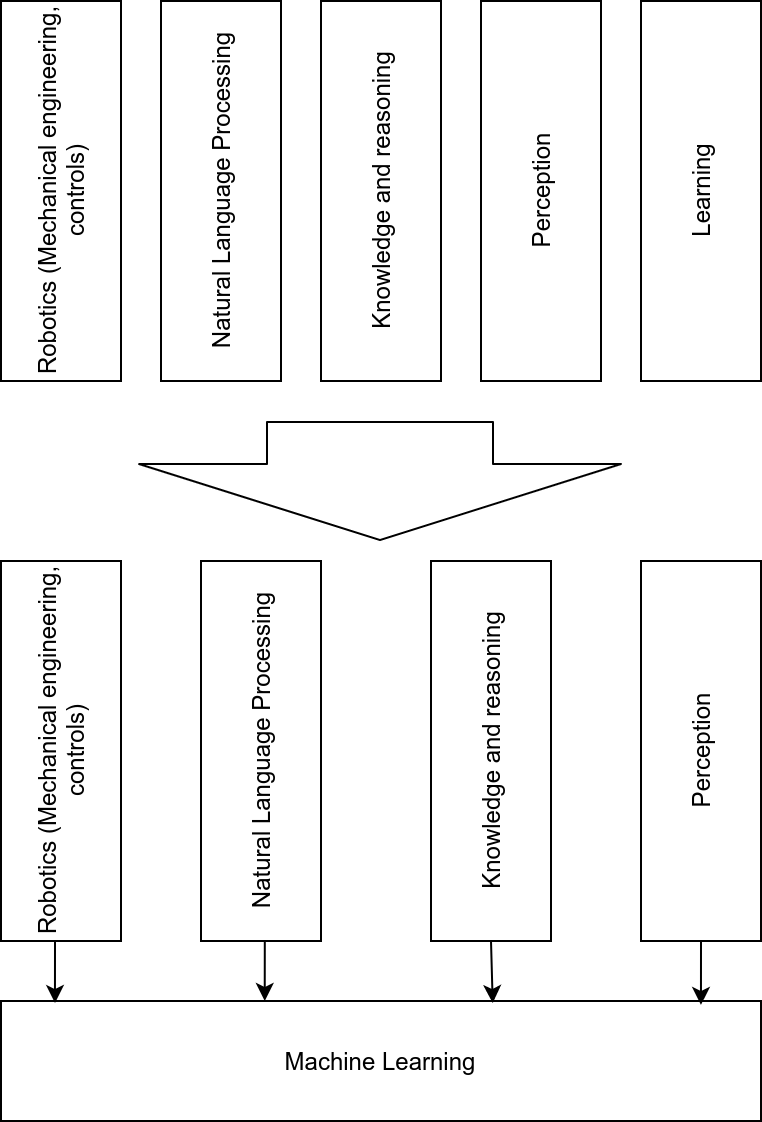
\includegraphics[width=.75\textwidth, center]{figures/agent_components_2}
			\end{figure}
		\end{column}
		\begin{column}{.5\textwidth}
			{\small 
				\begin{itemize}
					\item Image classification, localization and segmentation 
					\item Neural machine translation, question answering, summary. 
					\item Game playing, helicopter flying (stunts)
					\item Planning, self driving cars 
					\item Text, audio and video processing, generation 
					\item $\dots $
				\end{itemize}
			}
		\end{column}
	\end{columns}
\end{frame}
\begin{frame}{Machine learning models}
	\begin{columns}
		\begin{column}{.5\textwidth}
			\begin{block}{Models}
				\begin{itemize}
					\item Build a model of the world  
					\item Infer/predict using the model. 
				\end{itemize}
			\end{block}
		\end{column}
		
		\begin{column}{.5\textwidth}
			\begin{block}{Machine learning}			
				\begin{itemize}
					\item Supervised learning 
					\item Unsupervised learning 
					\item Reinforcement learning 
				\end{itemize}
			\end{block}
		\end{column}
	\end{columns}
\end{frame}

\begin{frame}{Supervised learning}
	\begin{columns}
		\begin{column}{.5\textwidth}
			\begin{figure}
				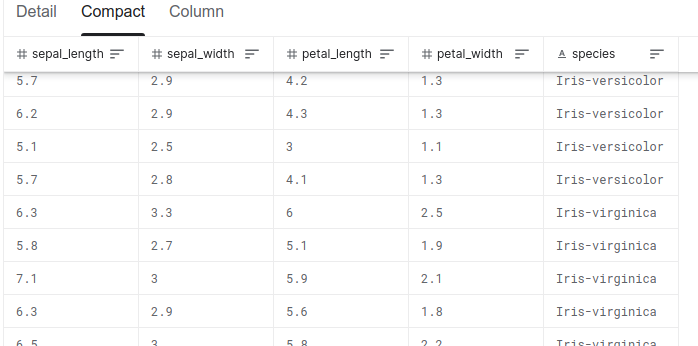
\includegraphics[width=1\textwidth, center]{figures/iris_dataset_1}
				
			\end{figure}
		\end{column}
		\begin{column}{.5\textwidth}
			\begin{figure}
				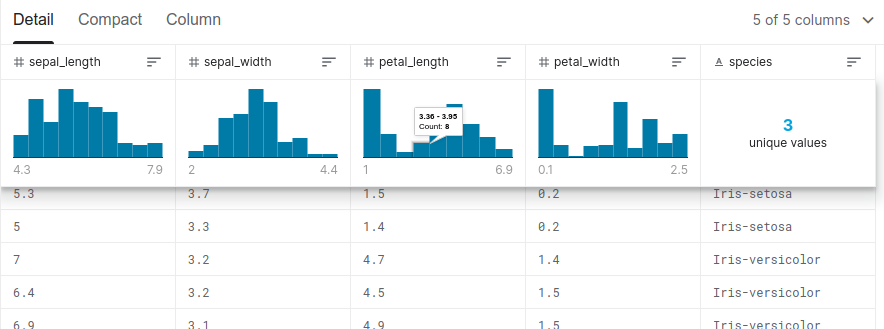
\includegraphics[width=1\textwidth, center]{figures/iris_dataset_2}
			
			\end{figure}
		\end{column}
	\end{columns}
	\begin{center}
		{\tiny Source:{\em https://www.kaggle.com/arshid/iris-flower-dataset?select=IRIS.csv}}
	\end{center}
\end{frame}

\begin{frame}{Supervised learning process flow}
	\begin{columns}
		\begin{column}{.5\textwidth}
			\begin{figure}
				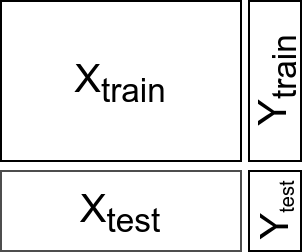
\includegraphics[width=.85\textwidth, center]{figures/ml_1_data}
				\caption*{Data}
			\end{figure}
		\end{column}
		\begin{column}{.5\textwidth}
			\begin{figure}
				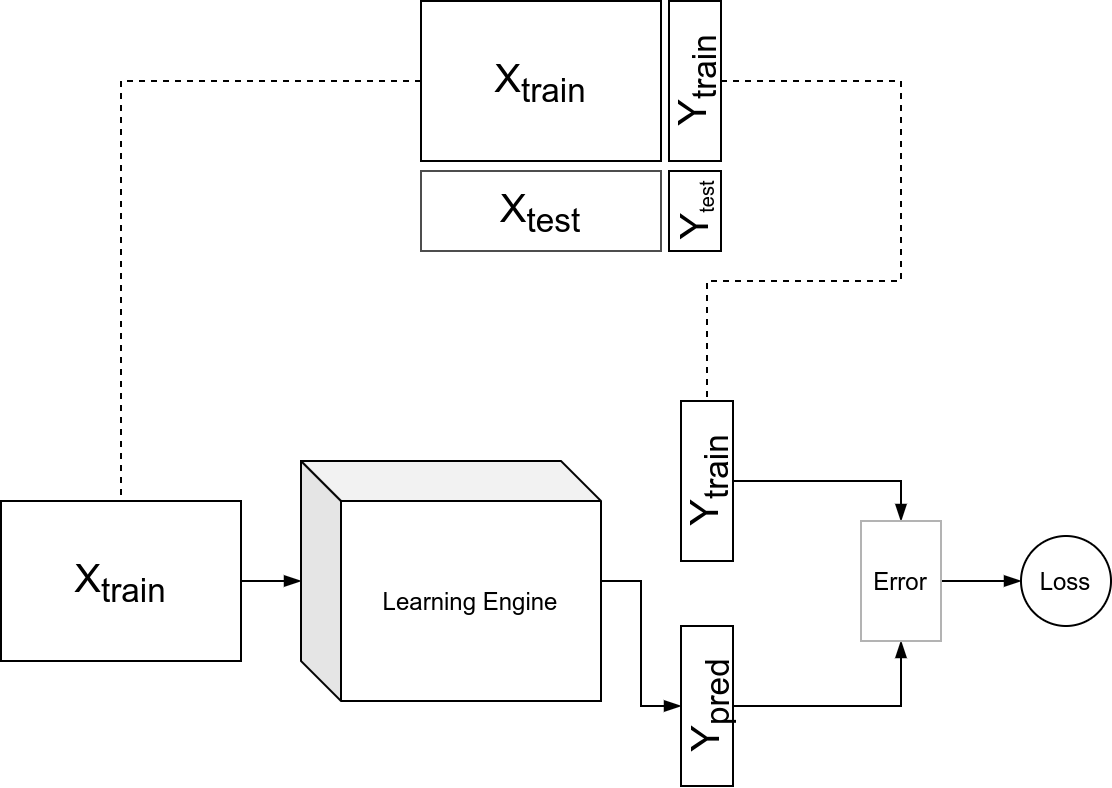
\includegraphics[width=1.\textwidth, center]{figures/ml_1_train}
				\caption*{Training}
			\end{figure}
		\end{column}
	\end{columns}
\end{frame}

\begin{frame}{Supervised learning process flow}
	\begin{columns}
		\begin{column}{.5\textwidth}
			\begin{figure}
				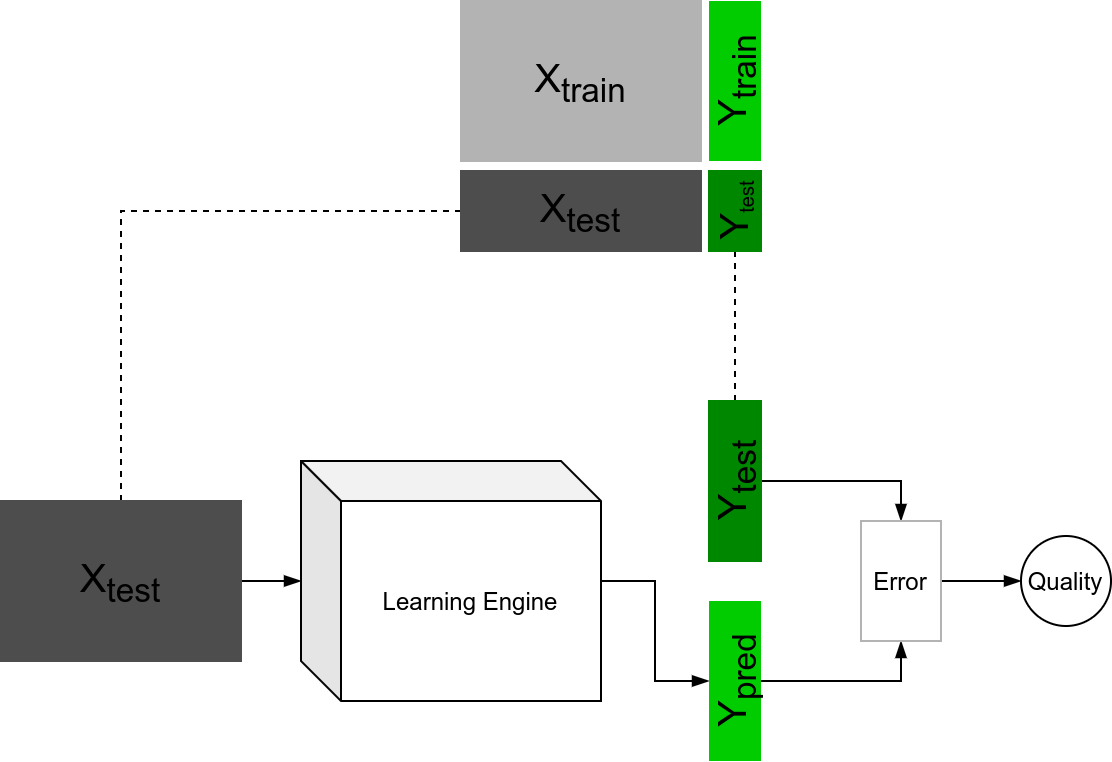
\includegraphics[width=1.\textwidth, center]{figures/ml_1_test}
				\caption*{}
			\end{figure}
		\end{column}
		\begin{column}{.5\textwidth}
			\begin{figure}
				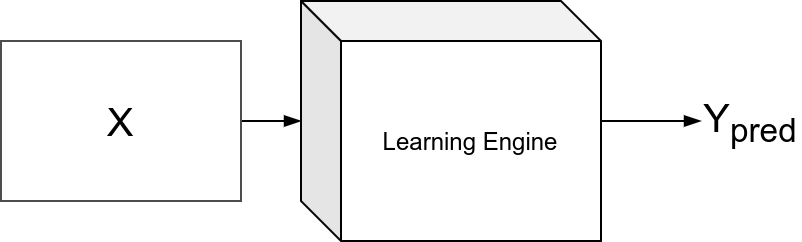
\includegraphics[width=1.\textwidth, center]{figures/ml_1_infer}
				\caption*{}
			\end{figure}
		\end{column}
	\end{columns}
	\begin{columns}
		\begin{column}{.5\textwidth}
			\begin{center}
				Testing
			\end{center}
		\end{column}
		\begin{column}{.5\textwidth}
			\begin{center}
				Predicting
			\end{center}
		\end{column}
	\end{columns}
\end{frame}


\begin{frame}{Machine learning}
	\begin{columns}
		\begin{column}{.5\textwidth}
			\begin{block}{Unsupervised learning}
				\begin{itemize}
					\item Training a model to find patterns in a dataset, typically an unlabeled dataset.
					\item Learning how to extract {\em interesting} features.
					\item Learning data distribution for generating data.
				\end{itemize}
			\end{block}
		\end{column}
		\begin{column}{.5\textwidth}
			\begin{block}{Reinforcement learning}
				A family of algorithms that learn an optimal policy, whose goal is to maximize return when interacting with an environment. 
				\begin{figure}
					
\includegraphics[width=.4\textwidth, center]{figures/RL_1}
				\end{figure}
			\end{block}
		\end{column}
	\end{columns}
\end{frame}
\section{A little bit of math}

\begin{frame}{Composition of functions} 
	\begin{columns}
		\begin{column}{.5\textwidth} 
			\begin{align}
				f(x)=& ax+b \\
				g(x)=&  \frac{1}{e^{-x}+1} \\
				g(f(x)) =& \frac{1}{e^{-(ax+b)}+1}   
			\end{align}
		\end{column}
		\begin{column}{.5\textwidth}
			\begin{figure}
				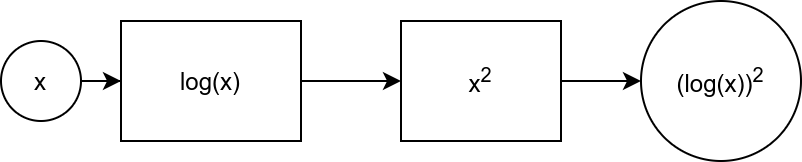
\includegraphics[width=.8\textwidth, center]{figures/function_composition}
				\caption*{Composite}
			\end{figure}
		\end{column}
	\end{columns}
\end{frame}

\begin{frame}{Derivatives}
	\begin{columns}
		\begin{column}{.5\textwidth}
			\begin{align}
				f(x)=&ax+b \\
				\frac{df(x)}{dx} =& a \\
				\sigma(z) =&\frac{1}{e^{-z}+1} \\
				\frac{d\sigma(z)}{dz} =& \sigma(z)(1-\sigma(z)) \\
				\frac{d\sigma(f(x))}{dx}=&?
			\end{align}
		\end{column}
		\begin{column}{.5\textwidth}
			\begin{figure}
				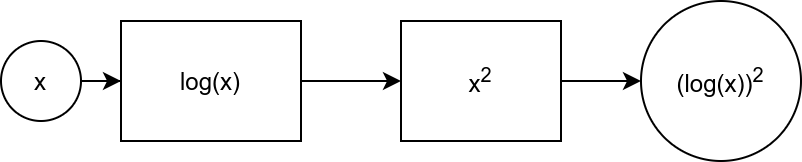
\includegraphics[width=.8\textwidth, center]{figures/function_composition}
				\caption*{Composite}
			\end{figure}
		\end{column}
	\end{columns}
\end{frame}

\begin{frame}{Derivatives}
	\begin{columns}
		\begin{column}{.5\textwidth}
			\begin{align}
				z=&ax+b \\
				\frac{dz}{dx} =& a \\
				\sigma(z) =&\frac{1}{e^{-z}+1} \\
				\frac{d\sigma}{dz} =& \sigma(z)(1-\sigma(z)) \\
				\frac{d\sigma}{dx}=&\frac{d\sigma}{dz} \frac{dz}{dx} 
			\end{align}
		\end{column}
		\begin{column}{.5\textwidth}
			\begin{figure}
				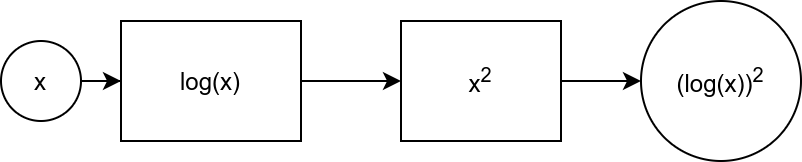
\includegraphics[width=.8\textwidth, center]{figures/function_composition}
				\caption*{Composite}
			\end{figure}
		\end{column}
	\end{columns}
\end{frame}


\begin{frame}{}
	\begin{columns}
		\begin{column}{.5\textwidth}
			\begin{align}
				z=&ax+b \\
				\frac{dz}{dx} =& a \\
				\sigma(z) =&\frac{1}{e^{-z}+1} \\
				\frac{d\sigma}{dz} =& \sigma(z)(1-\sigma(z)) \\
				\frac{d\sigma}{dx}=&\frac{d\sigma}{dz} \frac{dz}{dx}=\frac{dz}{dx} \frac{d\sigma}{dz}  
			\end{align}
		\end{column}
		\begin{column}{.5\textwidth}
			\begin{figure}
				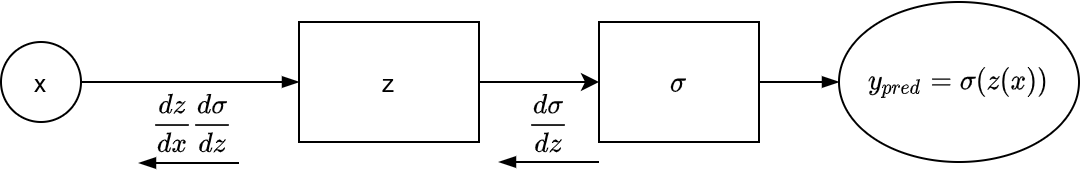
\includegraphics[width=.8\textwidth, center]{figures/function_composition_sigma}
				\caption*{Back propagation of gradients}
			\end{figure}
		\end{column}
	\end{columns}
\end{frame}
\section{Fitting functions}

\begin{frame}{Fitting a function to data}
		\begin{block}{Description (supervised learning)}
		Given a set of data $(x_1,y_1),(x_2,y_2), \dots, (x_n,y_n)$, can 
		we find a function $y=f(x)$ that "fits" this data? 		
		\end{block}		
		\begin{block}{Questions}
			\begin{itemize}
				\item What is this function $f(x)$?
				\item What does "fit" mean? 
				\item How do we know this works? 
				\item What kinds of problems can we solve? 
			\end{itemize}
		\end{block}
\end{frame}

\begin{frame}{More about $f(x)$}
	\begin{block}{Class of functions} 
		Starting with a function $f(x;\theta_1,\theta_2,\dots, \theta_n)$
		where $x$ is the input to the function and $\theta s$ are its parameters, 
		we need to find the set of $\theta s$ that best "fits" the give 
		data $(x_1,y_1),(x_2,y_2), \dots, (x_n,y_n)$ 
		
	\end{block}
	\begin{block}{Class of linear functions}
		Consider  $f(x) = ax+b$. If we can say, with some confidence, that 
		our data is linearly related,  we need to find  
		$\theta_1=a$, $\theta_2=b$ that {\it fits} the given data. 
		We can also write it as $f(x;a,b) = ax+b$. 
	\newline 
	Preferred,  
	\begin{align}
	f(x;\theta_1,\theta_2) &= \theta_1x+\theta_2	
	\end{align}

	\end{block}

\end{frame}
\begin{frame}{Fit}
	\begin{block}{Mean squared Euclidean distance as one possible measure of fit}
		Let $L_i$ be the squared Euclidean distance between the predicted 
		value, $\hat{y_i}=f(x_i)$ and the actual, $y_i$. Then,  
		\begin{align}
		L_i &=z_i^2 \\
		z_i &=y_i-f(x_i)\\
		    &=y_i-\theta_1 x_i-\theta_2 
		\end{align}
		Minimizing $L_i$ with respect to the parameters $\theta_1$ and $\theta_2$,
		\begin{align}
		\frac{\partial L_i}{\partial \theta_1} &= 
		\frac{\partial z_i^2}{\partial z_i} \; 
		\frac{\partial z_i}{\partial \theta_1}  \\
		\frac{\partial L_i}{\partial \theta_2} &= 
		\frac{\partial z_i^2}{\partial z_i} \; 
		\frac{\partial z_i}{\partial \theta_2} 
		\end{align}
	\end{block}
\end{frame}

\begin{frame}%{Mean squared distance and fit}
	For $n$ data points, mean  loss is 
	\begin{align*}
		L = \frac{1}{n} \sum_{i=1}^{i=n}L_i  
		  = \frac{1}{n} \sum_{i=1}^{i=n} (y_i-\theta_1 x_i-\theta_2)^2
	\end{align*}
	In practice
	\begin{itemize}
		\item Choose a small (64 or 128) random subset of training data. 
		\item Compute predicted values, then loss.
		\item Compute gradients of parameters W.R.T. loss and update parameters. 
	\end{itemize}
	An  {\bf epoch} refers to a single iteration over all training data.
	\begin{block}{Two different spaces}
		\begin{itemize}
			\item Space spanned by $x$ and $y$. Optimization tries to find the surface (model) 
			in this space that best fits the data. 
			\item Space spanned by $\theta s$. We minimize the loss function in this space.  
		\end{itemize}
	\end{block}
\end{frame}



%\section{Transfer learning, auto-encoders}

\begin{frame}{Transfer learning - image classification with CNN}
\begin{itemize}
	\item Earlier layers in convolution networks extract generic features (edges etc.)
	\item Layers get more specialized towards the end
	\item Training can take weeks. A trained model represents significant effort
	from experts. 
\end{itemize}
	\begin{center}
		\begin{figure}
			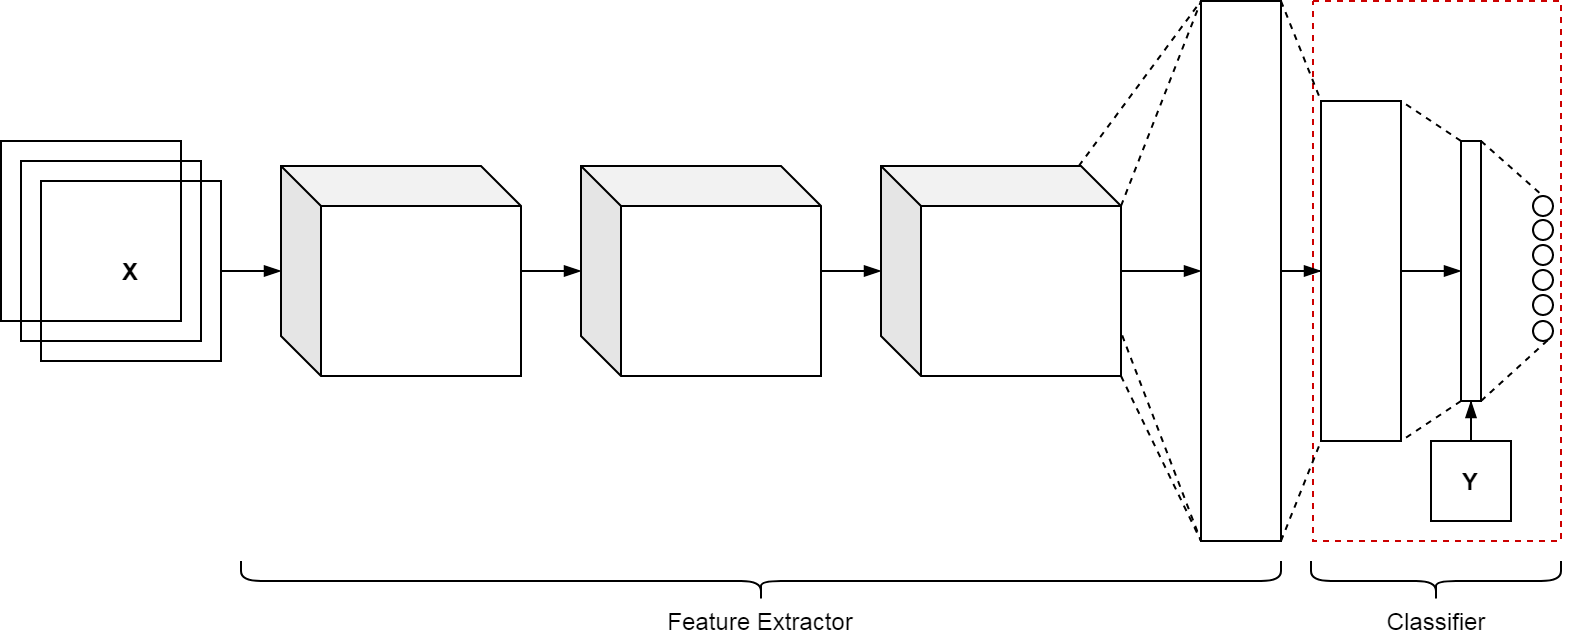
\includegraphics[width=.7\textwidth]{figures/deep_cnn_transfer_learning_1}
		\end{figure}
	\end{center}
\end{frame}
\begin{frame}{Transfer learning}
	\begin{center}
		\begin{figure}
			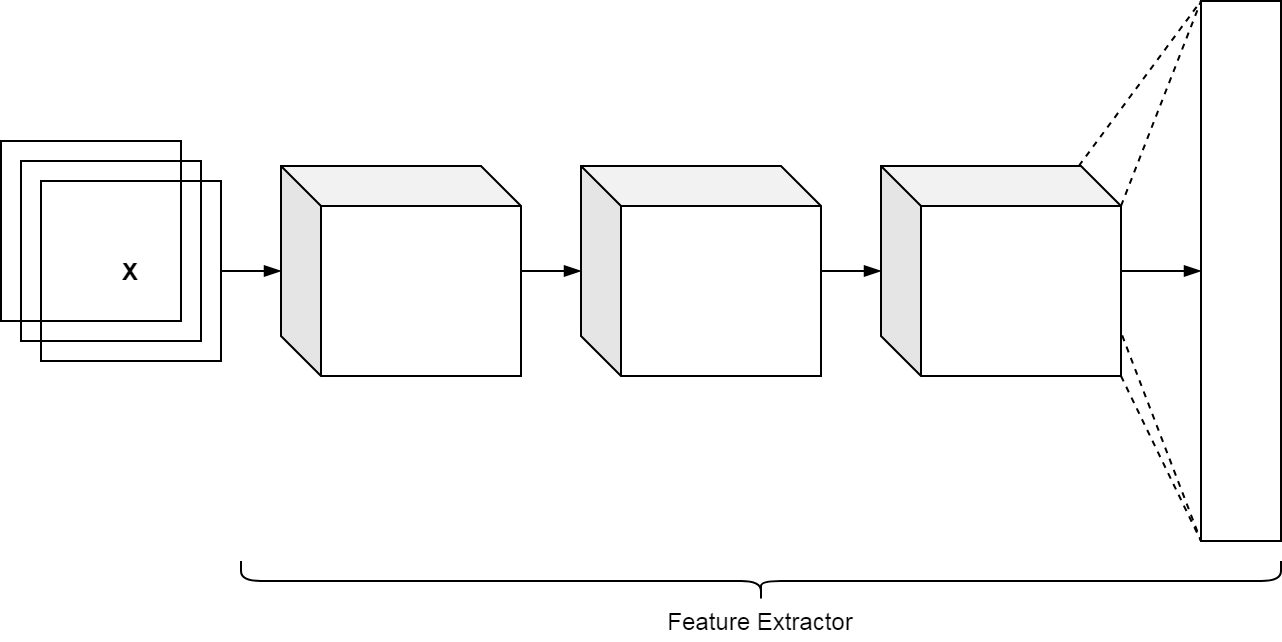
\includegraphics[width=1\textwidth]{figures/deep_cnn_transfer_learning_2}
		\end{figure}
	\end{center}
\end{frame}
\begin{frame}{Transfer learning}
	\begin{center}
		\begin{figure}
			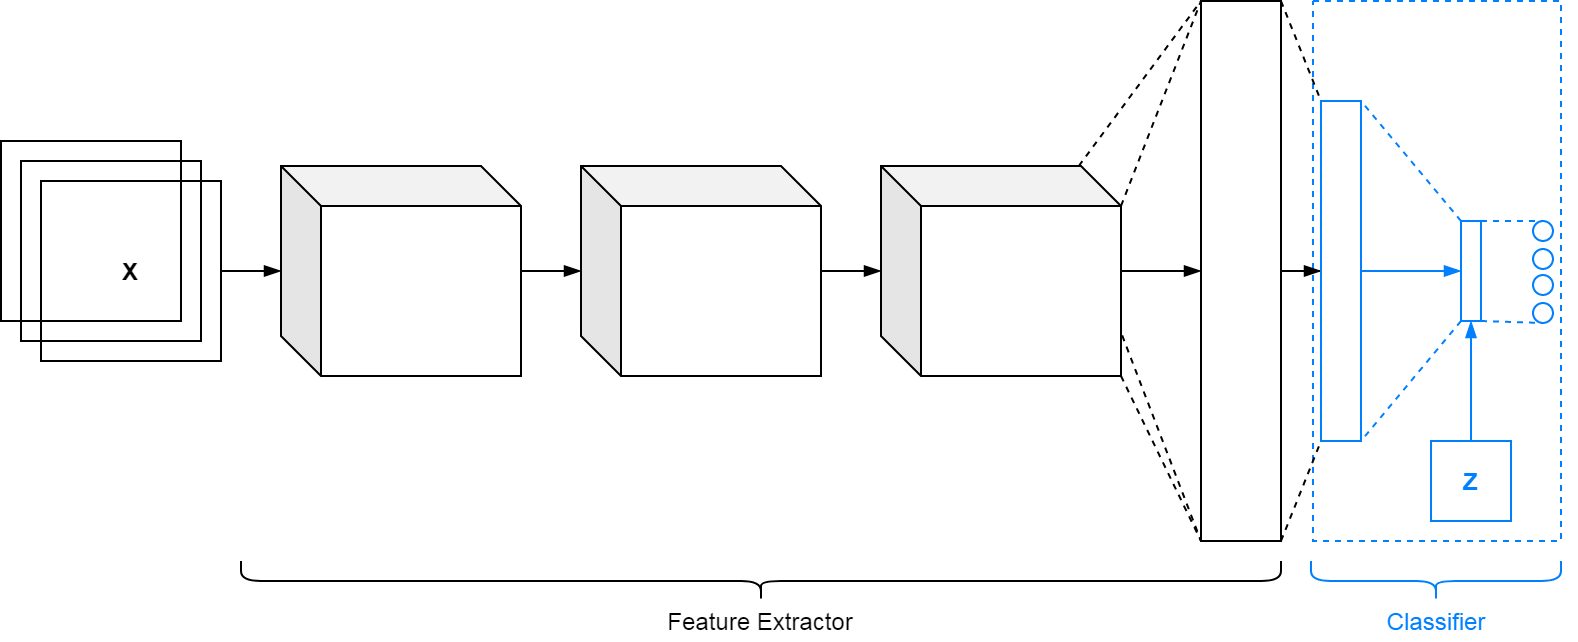
\includegraphics[width=1\textwidth]{figures/deep_cnn_transfer_learning_3}
		\end{figure}
	\end{center}
\end{frame}
\begin{frame}{Transfer learning - pytorch}
\begin{lstlisting}[language=Python,caption={Using pretrained ResNet18},captionpos=b]

import torch.nn as nn
from torchvision import datasets, models, transforms

model = models.resnet18(pretrained=True)
num_ftrs = model_ft.fc.in_features

# Here the size of each output sample is set to 2.
model.fc = nn.Linear(num_ftrs, 2)

\end{lstlisting}

\begin{lstlisting}[language=Python,caption={Freezing model parameters},captionpos=b]
for param in model.parameters():
  param.requires_grad = False
  
num_ftrs = model_ft.fc.in_features
model.fc = nn.Linear(num_ftrs, 2)
\end{lstlisting}

\end{frame}

\begin{frame}{Auto-encoders and approximate identity function}
\begin{itemize}
	\item Let us consider $y=f(x)$ as the network function. 
	\item Let us consider another network function $z=g(y)$ and $z$ has same shape as $x$.
	\item Let us consider a loss function, $L(x,g(f(x))$. This could be 
	\begin{itemize}
		\item[-] Squared distance $\frac{1}{n}\sum\limits_{i}(x_i-z_i)^2  $
		\item[-] Absolute difference $\frac{1}{n}\sum\limits_{i}|x_i-z_i|$
		\item[-] "Some" other distance metric between vectors in "some" latent space 
	\end{itemize}  
\end{itemize}
	\begin{figure}
		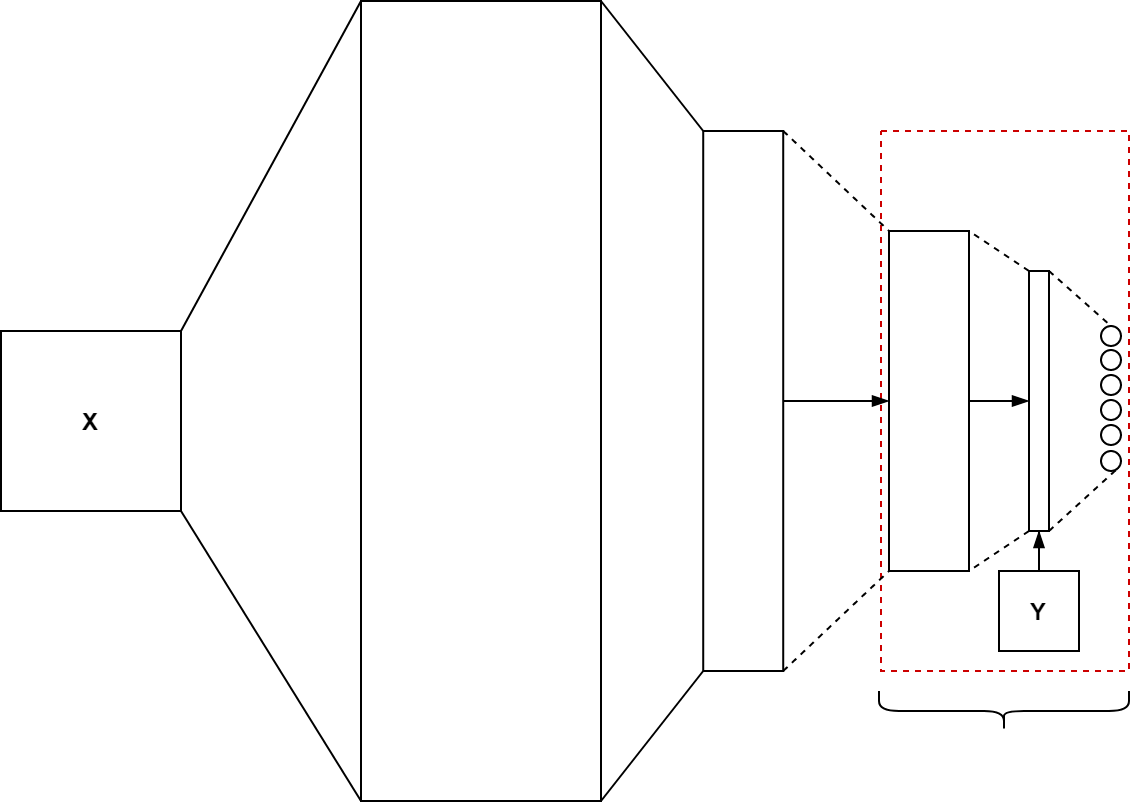
\includegraphics[width=.2\textwidth]{figures/autoencoder_1}
		\caption*{\tiny{$y=f(x)$}}
	\end{figure}
\end{frame}
\begin{frame}{Autoencoders and identity function} 
	\begin{center}
		\begin{figure}
			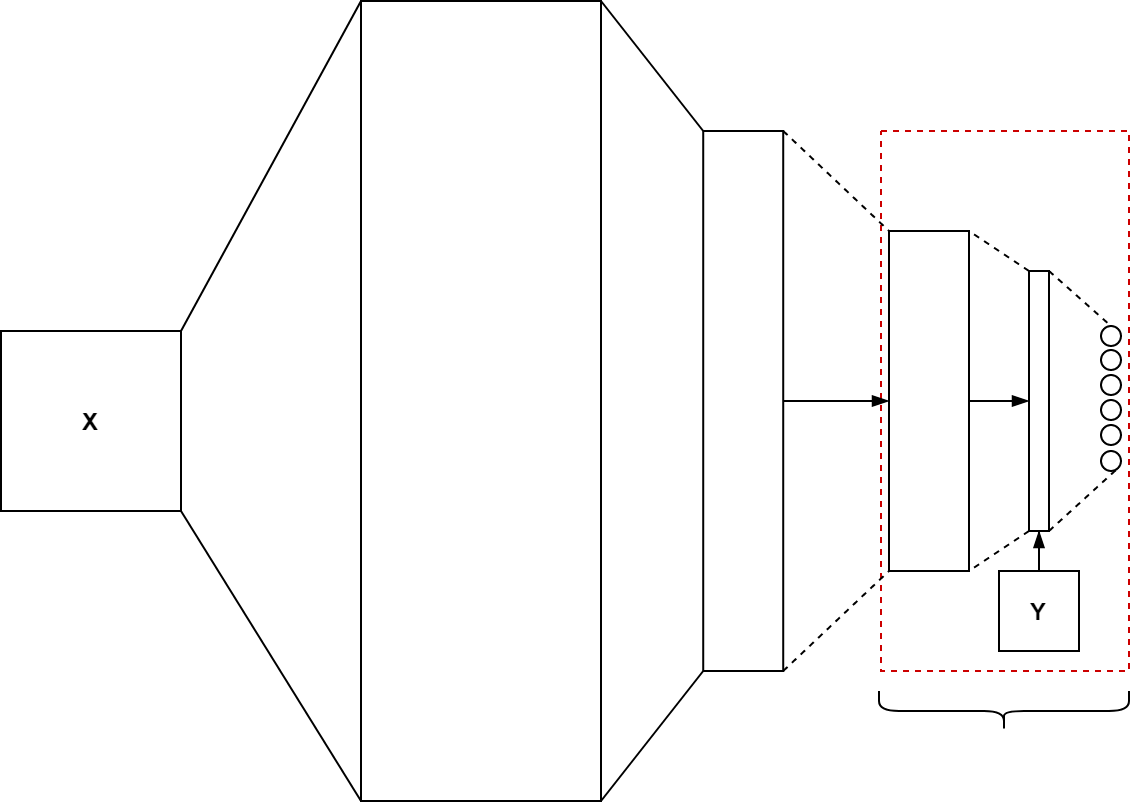
\includegraphics[width=.8\textwidth]{figures/autoencoder_1}
		\end{figure}
	\end{center}
\end{frame}
\begin{frame}{Autoencoders and identity function} 
	\begin{center}
		\begin{figure}
			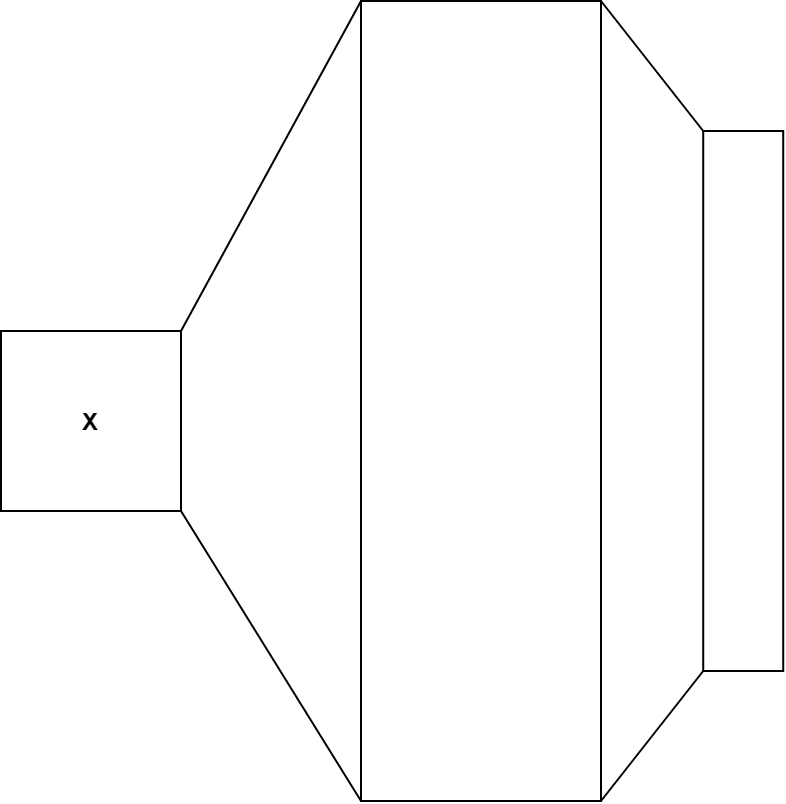
\includegraphics[width=.5\textwidth]{figures/autoencoder_2}
		\end{figure}
	\end{center}
\end{frame}
\begin{frame}{Autoencoders and identity function} 
	\begin{center}
		\begin{figure}
			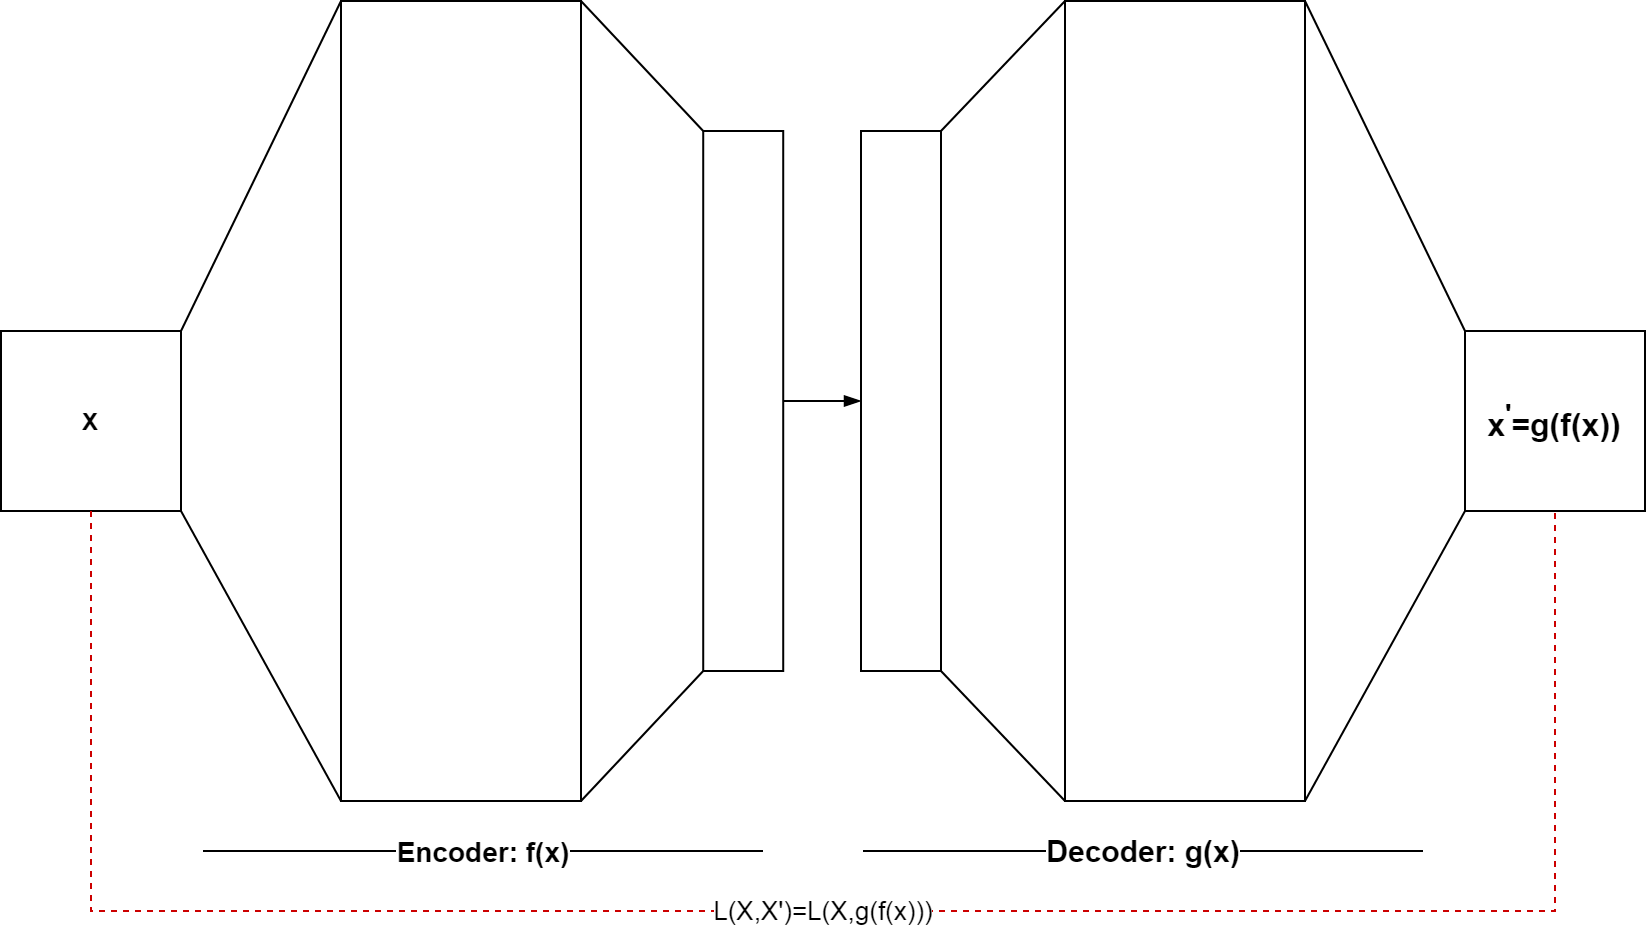
\includegraphics[width=.9\textwidth]{figures/autoencoder_3}
		\end{figure}
	\end{center}
\end{frame}

%\section{Recurrent networks and sequences}

\begin{frame}{Sequences} 
	%\begin{columns}
	%	\begin{column}{.5\textwidth}
			\begin{itemize}
				\item Natural language tasks 
				\item Event processing  
				\item Statefull systems in general
			\end{itemize}	
	%	\end{column}
	%	\begin{column}{.5\textwidth}
		\begin{block}{Types}
			\begin{itemize}
				\item Variable length sequences, all elements known ahead of time. 
				\item Constant length sequences, all elements known ahead of time. 
				\item Constant length sequences, revealed one element at a time.
				\item Variable length sequences, revealed one element at a time.
			\end{itemize}
		\end{block}

	%	\end{column}
	%\end{columns}
\end{frame}

\begin{frame}{Functions of form $y_t = f(y_{t-1}, x_t; \theta)$}

\begin{eqnarray}
I_t =& UX+Vh_{t-1}+b \\
h_t =& tanh(I_t) \\
O_t =& Wh_t + c 
\end{eqnarray}

\begin{center}
\begin{figure}
	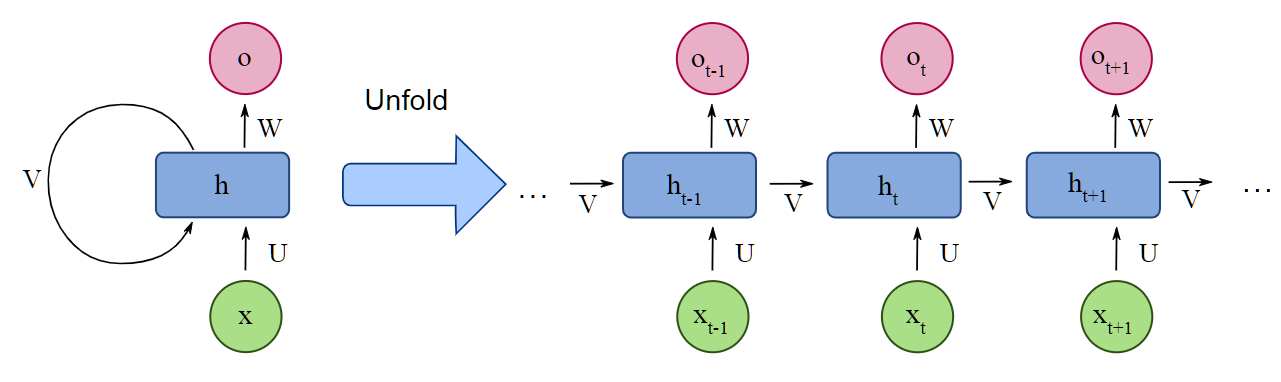
\includegraphics[width=.8\textwidth]{figures/rnn_wikipedia_1}
	\caption*{\tiny{"Recurrent neural network" (2020) Wikipedia. Available at:
	https://en.wikipedia.org/wiki/Recurrent\_neural\_network}}
\end{figure}
\end{center}
\end{frame}

\begin{frame}{Recurrent network architecture styles}
\begin{center}
	\begin{figure}
		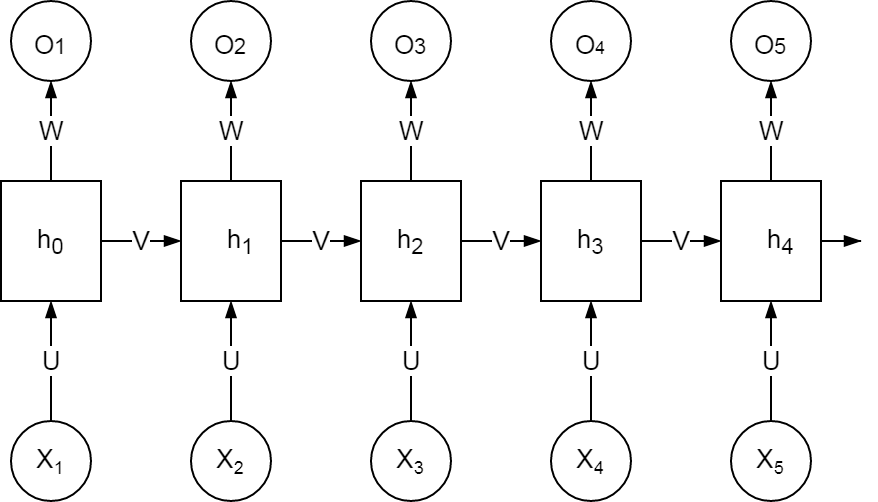
\includegraphics[width=1\textwidth]{figures/rnn_seq_2_seq}
		\caption*{{Sequence to sequence network}}
	\end{figure}
\end{center}
\end{frame}
\begin{frame}{Recurrent network architecture styles}
\begin{center}
	\begin{figure}
		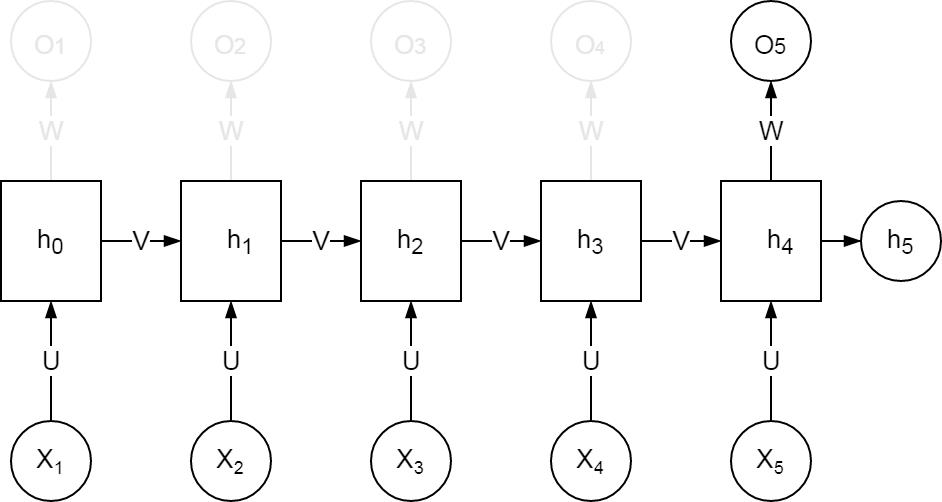
\includegraphics[width=1\textwidth]{figures/rnn_seq_2_vec}
		\caption*{{Sequence to vector network}}
	\end{figure}
\end{center}
\end{frame}
\begin{frame}{Recurrent network architecture styles}
\begin{center}
	\begin{figure}
		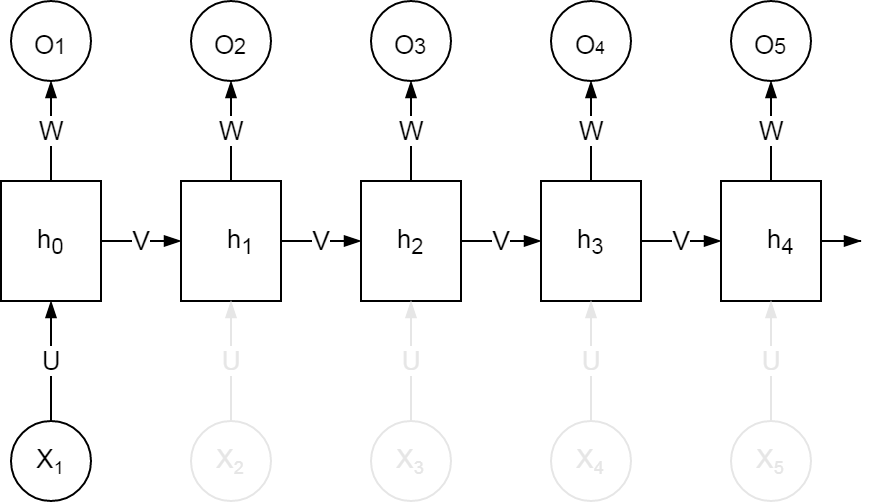
\includegraphics[width=1\textwidth]{figures/rnn_vec_2_seq}
		\caption*{{Vector to sequence network}}
	\end{figure}
\end{center}
\end{frame}
\begin{frame}{Recurrent network architecture styles}
\begin{center}
	\begin{figure}
		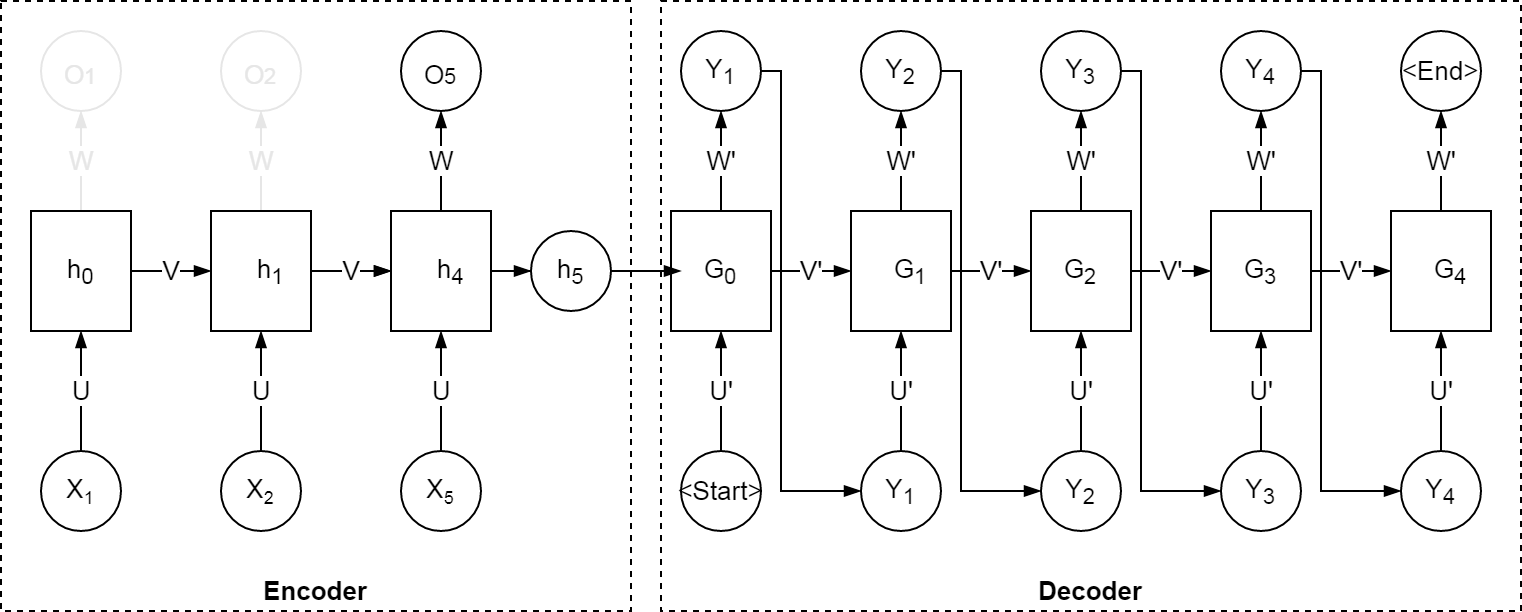
\includegraphics[width=1\textwidth]{figures/rnn_seq_2_seq_encoder_decoder}
		\caption*{{Sequence to sequence encoder-decoder network}}
	\end{figure}
\end{center}
\end{frame}
%\section{Miscellaneous topics}

\begin{frame}{Adversarial attacks}
\begin{columns}
	\begin{column}{.5\textwidth}
		\begin{figure}
			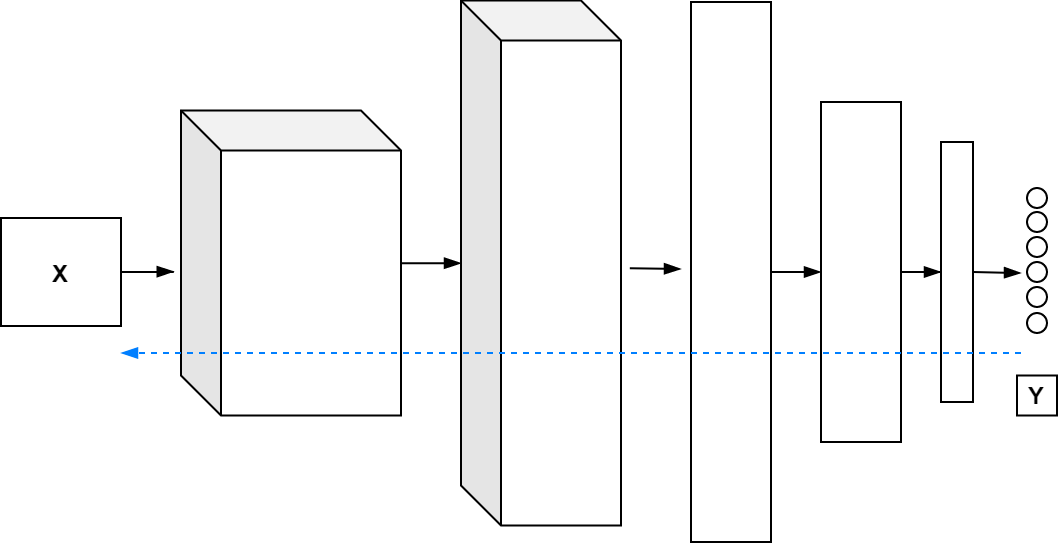
\includegraphics[width=1\textwidth]{figures/adverserial-net}
		\end{figure}
	\end{column}
	\begin{column}{.5\textwidth}
		Let $\hat{y}$ be desired,  $y$ be the predicted label, 
		and $\hat{x}$ be the desired image 
		\begin{enumerate}
			\item Simple loss function, $L=D(\hat{y},y)$
			\item Another loss function, $L=D_1(\hat{y},y) + \lambda D_2(\hat{x},x) $
		\end{enumerate}
	\end{column}
\end{columns}
\end{frame}
\begin{frame}{Adversarial examples}
\begin{columns}
\begin{column}{.5\textwidth}
	\begin{figure}
		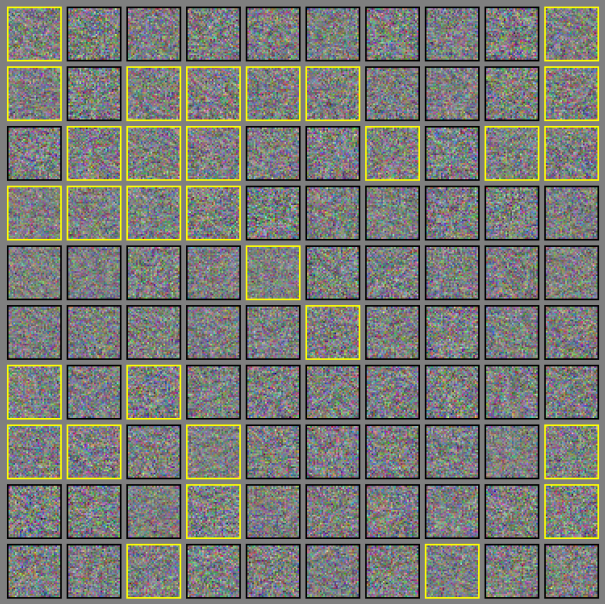
\includegraphics[width=.8\textwidth]{figures/adverserial-example-1}
		\caption*{\tiny{I. Goodfellow, J. Shlens, and C. Szegedy, Explaining and
				harnessing adversarial examples," in International Conference on Learning Representations, 2015.}}
	\end{figure}
\end{column}
\begin{column}{.5\textwidth}
	\begin{figure}
		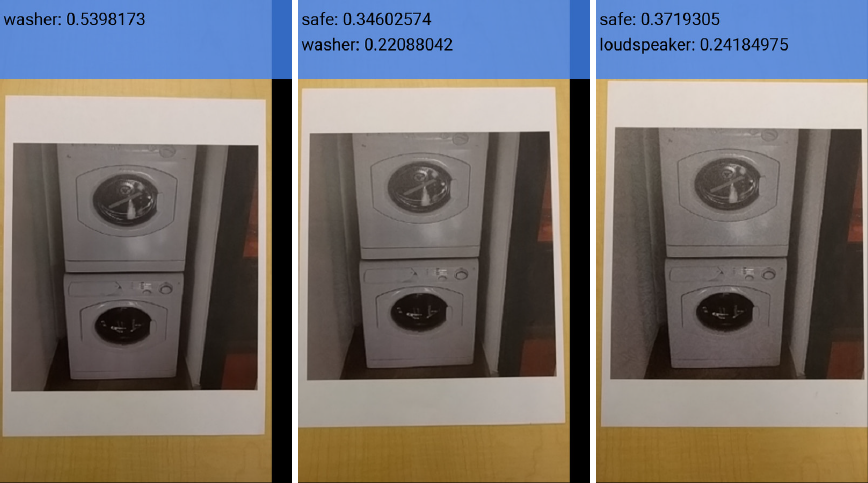
\includegraphics[width=1\textwidth]{figures/adverserial-example-2}
		\caption*{\tiny{A. Kurakin, I. Goodfellow, and S. Bengio, Adversarial
				examples in the physical world," ICLR Workshop, 2017.}}
	\end{figure}
	What kinds of attacks can you think of?
\end{column}
\end{columns}
\end{frame}

\begin{frame}{Generative adversarial networks - intuition}
\begin{center}
	\begin{figure}
		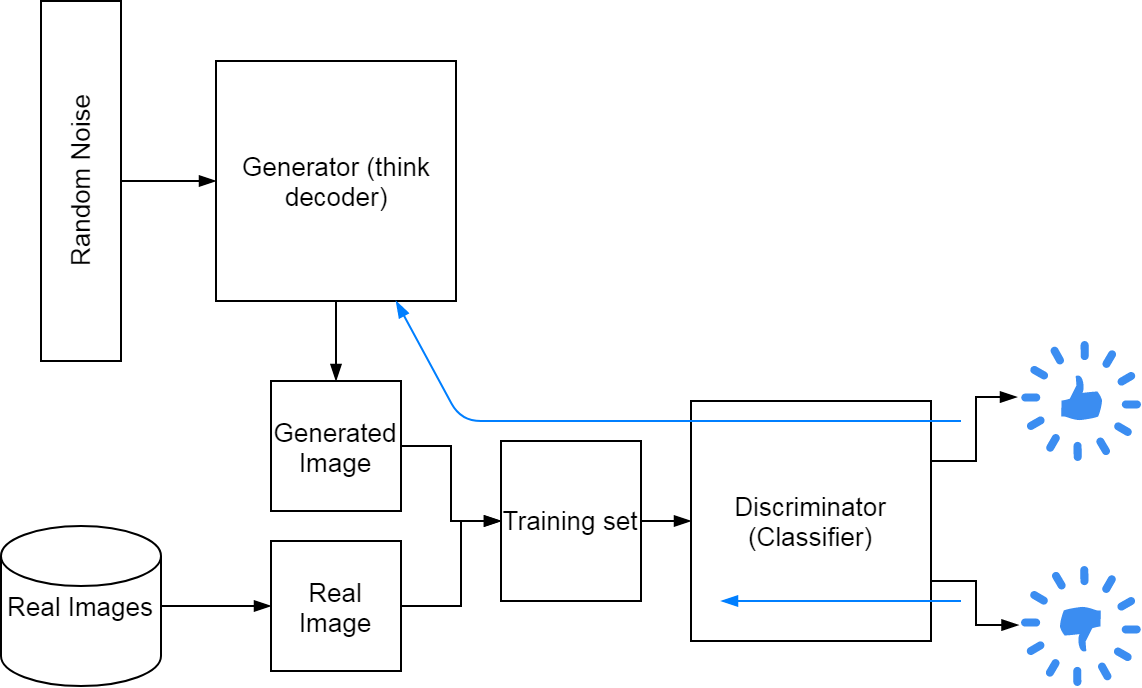
\includegraphics[width=1\textwidth]{figures/gan-simple}
	\end{figure}
\end{center}
\end{frame}

\begin{frame}{Attention - intuition} 
\begin{center}
	\begin{figure}
		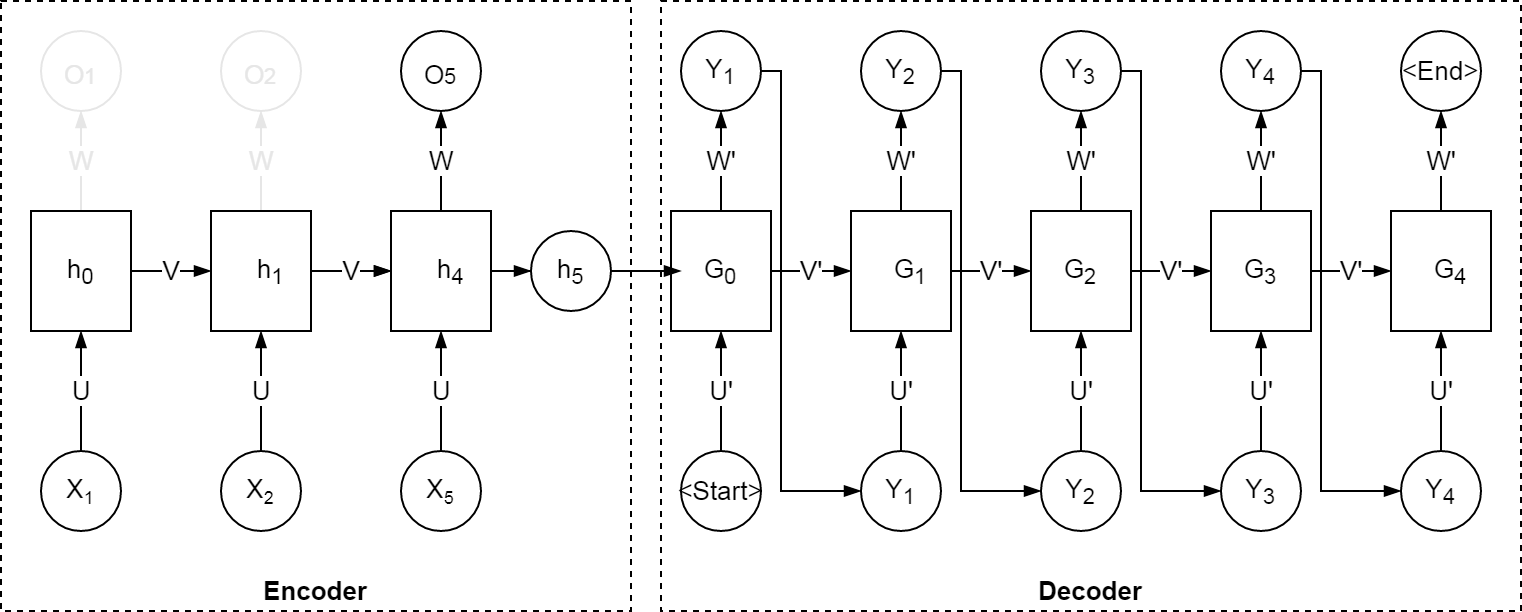
\includegraphics[width=1\textwidth]{figures/rnn_seq_2_seq_encoder_decoder}
		\caption*{{Sequence to sequence encoder-decoder network}}
	\end{figure}
\end{center}
\end{frame}
\section{References}
\begin{frame}
\frametitle{References}
\footnotesize{
	\begin{thebibliography}{99}
		\bibitem[Baydin 2018]{p1} Automatic differentiation in machine learning: A survey\\
		\newblock Atilim Gunes Baydin, Barak A. Pearlmutter \& Alexey Andreyevich Radul
		\newblock \emph{arxiv} http://arxiv.org/abs/1502.05767
		
	\end{thebibliography}
}
\end{frame}



\end{document}
